\begin{figure*}[t]
    \centering
       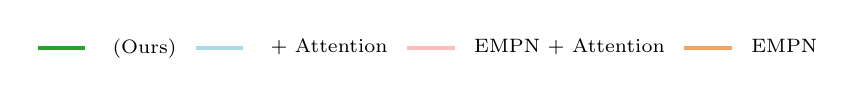
\begin{tikzpicture}
    \tikzstyle{every node}=[font=\scriptsize]
    \definecolor{tabblue}{RGB}{31, 119, 180}
\definecolor{taborange}{RGB}{255, 127, 14}
\definecolor{tabgreen}{RGB}{44, 160, 44}
\definecolor{tabred}{RGB}{214, 39, 40}
\definecolor{tabpurple}{RGB}{148, 103, 189}
\definecolor{tabbrown}{RGB}{140, 86, 75}
\definecolor{tabpink}{RGB}{227, 119, 194}
\definecolor{tabgray}{RGB}{127, 127, 127}
\definecolor{tabolive}{RGB}{188, 189, 34}
\definecolor{tabcyan}{RGB}{23, 190, 207}
\definecolor{lightblue}{RGB}{173, 216, 230}
\definecolor{sandybrown}{RGB}{244, 164, 96}
\definecolor{darkgrey}{RGB}{169, 169, 169}
\definecolor{dimgrey}{RGB}{105, 105, 105}
\definecolor{olivedrab}{RGB}{107, 142, 35}
\definecolor{darkviolet}{RGB}{148, 0, 211}
\definecolor{darkgoldenrod}{RGB}{184, 134, 11}
\definecolor{darkblue}{RGB}{0, 0, 139}
\definecolor{orchid}{RGB}{218, 112, 214}

    \begin{axis}[%
        hide axis,
        xmin=10,
        xmax=50,
        ymin=0,
        ymax=0.1,
        legend style={
            draw=white!15!black,
            legend cell align=left,
            legend columns=4,
            legend style={
                draw=none,
                column sep=1ex,
                line width=1pt,
            }
        },
        ]
        \addlegendimage{line legend, tabgreen, ultra thick} % Thicker line here
        \addlegendentry{\textbf{\model} (Ours)}
        \addlegendimage{line legend, lightblue, ultra thick} % Thicker line here
        \addlegendentry{\textbf{\model} + Attention}
        \addlegendimage{line legend, pink, ultra thick} % Thicker line here
        \addlegendentry{EMPN + Attention}
        \addlegendimage{line legend, sandybrown, ultra thick} % Thicker line here
        \addlegendentry{EMPN}
    \end{axis}
\end{tikzpicture}

        \centering
        \begin{subfigure}[b]{0.24\linewidth}
            \includegraphics[width=\textwidth]{ICLR_2025/Figures/eval_all_bar_6_tasks/consistent_eval_bar_Isaac-Rigid-Sliding-Multi-v0_eval_all.pdf}
        \end{subfigure}
        \hfill
        \begin{subfigure}[b]{0.24\linewidth}
            \includegraphics[width=\textwidth]{ICLR_2025/Figures/eval_all_bar_6_tasks/eval_bar_Isaac-Rigid-Insertion-Multi-v0_eval_consistent.pdf}
        \end{subfigure}
        \hfill
        \begin{subfigure}[b]{0.24\linewidth}
            \includegraphics[width=\textwidth]{ICLR_2025/Figures/eval_all_bar_6_tasks/eval_bar_Isaac-Rigid-Insertion-Multi-Two-Actuators-v0_eval_consistent.pdf}
        \end{subfigure}
        \hfill
        \begin{subfigure}[b]{0.24\linewidth}
            \includegraphics[width=\textwidth]{ICLR_2025/Figures/eval_all_bar_6_tasks/eval_bar_Isaac-Rigid-Pushing-No-Contact-Multi-v0_eval_all.pdf}
        \end{subfigure}

        % \vspace{-0.05cm}
        
        \begin{subfigure}[b]{0.24\linewidth}
            \includegraphics[width=\textwidth]{ICLR_2025/Figures/eval_all_bar_6_tasks/eval_bar_Isaac-Rope-Closing-v0_eval_all.pdf}
        \end{subfigure}
        \hfill
        \begin{subfigure}[b]{0.24\linewidth}
            \includegraphics[width=\textwidth]{ICLR_2025/Figures/eval_all_bar_6_tasks/eval_bar_Isaac-Rope-Shaping-v0_eval_all.pdf}
        \end{subfigure}
        \hfill
        \begin{subfigure}[b]{0.24\linewidth}
            \includegraphics[width=\textwidth]{ICLR_2025/Figures/eval_all_bar_6_tasks/eval_bar_Isaac-Cloth-Hanging-Multi-v0_eval_all.pdf}
        \end{subfigure}
        \hfill
        \begin{subfigure}[b]{0.24\linewidth}
            \includegraphics[width=\textwidth]{ICLR_2025/Figures/eval_all_bar_6_tasks/overhead_small.pdf}
        \end{subfigure}

    \captionof{figure}{Performance comparison on tasks with and without attention mechanisms over 10 seeds. Adding attention significantly increases the training time but does not improve performance, as shown on the right. The computational overhead is measured as the ratio of training time per iteration (over \rebuttal{seven} tasks) relative to HEPi.}
    \label{fig:eval_attention}
\end{figure*}
